% This is samplepaper.tex, a sample chapter demonstrating the
% LLNCS macro package for Springer Computer Science proceedings;
% Version 2.20 of 2017/10/04
%
\documentclass[runningheads]{llncs}
%
\usepackage{graphicx}
\usepackage{amssymb}
% Used for displaying a sample figure. If possible, figure files should
% be included in EPS format.
%
% If you use the hyperref package, please uncomment the following line
% to display URLs in blue roman font according to Springer's eBook style:
% \renewcommand\UrlFont{\color{blue}\rmfamily}

\begin{document}
%
\title{Coordinate Matrix Machine: An Augmented Intelligence Approach to Classify Very Similar Documents}
\titlerunning{Coordinate Matrix Machine}
%
%\titlerunning{Abbreviated paper title}
% If the paper title is too long for the running head, you can set
% an abbreviated paper title here
%
\author{Amin Sadri \and
M. Maruf Hossain\thanks{corresponding author}}
%
\authorrunning{Sadri and Hossain}
% First names are abbreviated in the running head.
% If there are more than two authors, 'et al.' is used.
%
\institute{Australia and New Zealand Banking Corporation\\
\email{\{sadria,maruf.hossain\}@anz.com}\\
\url{http://www.anz.com/}}
%
\maketitle              % typeset the header of the contribution
%
\begin{abstract}
Document classification, in general, focuses primarily on the context of the document and classify based on its belonging to one or more classes. However, if the documents are more structured and contains very similar content to one another, then traditional approaches do not yield the required high accuracy demanded by many applications.

\textbf{Contribution.} In this paper, we have proposed a coordinate matrix-based approach which augments human intelligence to create a very small vector to learn the structure of the document and use this information to classify the documents.

\textbf{Result.} The algorithm outperforms every popular vectoriser techniques in combination with traditional machine learning and most advanced deep learning models that rely on a larger number of elements to achieve good accuracy. The advantages of our algorithm are:
\begin{enumerate}
\item Better accuracy
\item Faster computation
\item Small memory footprint
\item Generic, expandable and extendable
\item Explainable
\item Robust against unbalanced classes
\item Does not require large number of labelled data
\end{enumerate}

\keywords{Augmented intelligence \and Coordinate Matrix \and Lazy Learning \and Classification.}
\end{abstract}
%
%
%
\section{Introduction}
Document classification is a common task in machine learning in the form of Natural Language Processing (NLP) where a document is assigned to one or more classes. Current approaches rely heavily on the context of the document in order to classify them~\cite{jones1972,power2010}. Identifying the relevant topic is the primary motivator for such document classification~\cite{hassan2017,kotenko2015,lin2006}. But what if there is a large number of structured documents that needs to be classified based on the originator or the structure of the document. For example, various bank statements received along with loan applications, where the task is to identify the issuing bank for those statements and to identify which existing function to employ to extract information from those statements, i.e., identify the template for the statement.

\subsection{Challenges}
There are several challenges when working with documents that are very similar in nature. We have identified the following challenges when dealing with bank statements.

\begin{itemize}
\item A large number of documents need to be labelled to train a model with sufficient accuracy, which is both time and resource consuming.
\item There are way too many class labels at the template level. For the five banks included in this experiment, there were 53 templates (classes) available.
\item There are not enough representative samples for each class.
\item All bank statements look very similar to one another.
\item Majority of the words in bank statements are personal and highly contextual, such as account holder's name, address or transaction items, which produces lots of noise when training a classification model.
\item The words which are not noise are very similar across a range of bank statements, e.g., ‘Name’, ‘Account’, ‘Balance’, ‘Date’.
\end{itemize}

Due to these challenges, traditional machine learning models and more recent deep learning models do not perform well. 
\begin{example}
While classifying statements for issuing banks Term Frequency vectoriser with Logistic Regression has an $F$-measure of 1.0, but the value dropped to 0.79 when we attempted to classify templates. 
\end{example}

This lower performance can discourage users to use simplistic models and inclined to use more complex models like Convolutional Neural Network (CNN) or Recurrent Neural Network (RNN)~\cite{banerjee2019,kumar2019}, which are by default not explainable, and rely on additional techniques~\cite{ribeiro2016} to explain, especially to the governing body for compliance purpose.
\begin{example}
But after running hours to build CNN or Long Short-Term Memory (LSTM) RNN architecture, we have found that CNN has a $F$-measure of 0.99, while LSTM only has 0.67 while classifying the issuing banks of the statements. To classify 53 templates the performance is equally lower than that of our simple Logistic Regression model.
\end{example}

\subsection{Our Contribution}
\textit{Our aim in this paper is to improve the classification performance on high number of classes when the documents are very similar to one another, by incorporating domain knowledge to create a small input vector so that neither inducing the model nor applying the model takes very long time.}

In this paper, we have proposed a novel classification approach which augments human intelligence~\cite{zheng2017} to create a very small input vector. This allows us to learn the structure of the document and use this information for document classification. The proposed model is based on creating a coordinate matrix for the input terms.

In short, we have developed a hybrid lazy learning algorithm, Coordinate Matrix Machine (CM$^2$), to create an input matrix (which contrasts with traditional vector-based input strategy) and use this matrix to classify documents.

The rationale behind the technique are as follows:
\begin{remark}
With structured documents, the position carries more importance than the occurrence or the order of the occurrence for the terms. Furthermore, by augmenting the understanding of the subject matter experts, we can avoid developing huge corpus to improve classification performance.
\end{remark}

\begin{remark}
This technique would allow us to avoid labelling large amount of documents often needed to train machine learning and deep learning models.
\end{remark}

\subsection{Advantages}
The advantages of our algorithm are:
\begin{enumerate}
\item It has better accuracy compared to all algorithms tested.
\item It has faster computation.
\item It has a very small memory footprint.
\item It is generic, expandable and extendable. For newer samples, there is no need for any feature engineering or feature extraction.
\item It is explainable. It is easy to trace the reason behind classification and modify, if necessary. 
\item It is not affected by unbalanced classes, low-volume or low-quality training data.
\item It does not require large number of labelled data.
\end{enumerate}

\subsection{Organisation}
The remainder of the paper is organised as follows. In Section~\ref{work}, we briefly discuss the related work in document classification. Our algorithm is formally described in Section~\ref{algo}. Section~\ref{exp} presents the design of the experimental investigation. We present and discuss the results in Section~\ref{result} and~\ref{discuss}. Finally, in Section~\ref{conc}, we suggest future improvements and conclude the paper.

\section{Related Work}\label{work}
As document classification has become an emerging area in the text mining research, a large amount of prior work has focused on it. A typical document classification has several pre-processing steps and researches focused on each step to improve the performance, such as stopwords removal~\cite{manalu2017,prathibha2015}, Tokenization~\cite{bakar2014,gadri2015}, Part-of-Speech Tagging~\cite{owoputi2012}, Stemming~\cite{zhang2007}.

The second step usually focus on feature extraction and selection. For example, Yang et al.~\cite{yang2002} used titles and other tag data to label the text features. Shih and Karger~\cite{shih2004} used the geometry of the rendered HTML page to build up tree models based on the incoming link structure. Term Frequency–Inverse Document Frequency (TF-IDF) is a popular way for feature selection~\cite{jones1972}. Power et al.~\cite{power2010} focused on web page classification and filtered the output of the TF-IDF algorithm to improve the performance.

Once the feature vector is identified, the third step is to apply a machine learning model for classification. Na\"ive Bayes is one of the probability-based classifiers~\cite{kotenko2015}. Decision tree-based approaches have also been used for different purposes such as inappropriate web content blocking~\cite{liu2017}. Support Vector Machines (SVM) are also widely used for document classification~\cite{farhoodi2010,lin2006}. There are multiple approaches under artificial/deep neural network. Hassan and Mahmood~\cite{hassan2017} applied Convolution Neural Networks (CNN) for document classification. Unlike most of the machine learning models, Recurrent Neural Networks (RNN) take the sequence of the occurrences of the words into consideration, therefore documents with similar words will have different outputs because of the order of the words~\cite{banerjee2019,kumar2019}.

\section{Methodology}\label{algo}
We now describe in more detail, the steps in our algorithm for creating the feature vector and inducing the classifier using the coordinate matrix.

\subsection{Pre-processing the Documents}
Each training data is a PDF file contains either a scanned image or a digital document. We have ensured that each page of the document is set to 300 dpi before we run the pages through an Optical Character Reader (OCR) engine to get the words and their respective coordinates. The output of the OCR is stored as eXtensible Mark-up Language (XML) files that are used as input to induce our model.

\subsection{Building the Coordinate Matrix}
For each class, only one sample is required for training. We accompany a Comma Separated Value (CSV) files with each XML file, which contains key-value pair for all entities within the document.
\begin{example}
Statement A contains the term `Account Number’ followed by the account number `061234-12345678’, the term `Account Holder’ with the value `John Doe’, and the term `Account Type’ with the value `Savings Account’. Whereas, in statement B, the relevant term `Account No.’ followed by the number `064321-87654321’, and the term `Account Name’ with the value `Jane Smith’ is recorded. So in the CSV file for statement A, we have the entries ``\texttt{Account Number,061234-12345678}'', ``\texttt{Account Holder, John Doe}'' and ``\texttt{Account Type,\\Savings Account}''; and for statement B, we have ``\texttt{Account No.,064321-\\87654321}'' and ``\texttt{Account Name,Jane Smith}'' recorded.
\end{example}

We then search for the keys and their corresponding values in the XML and construct a matrix with top, left, bottom and right position of the labels for each key for each document as shown in Tab.~\ref{matrix}. We search for both key and value in the close proximity to avoid picking up other similar labels that is available in the statement.
\begin{table}
\centering
\caption{Example of the Coordinate Matrix}\label{matrix}
\begin{tabular}{|l|l|r|r|r|r|}
\hline
Document ID & Key & Top & Left & Bottom & Right\\
\hline
Statement A & Account Number & 254 & 1231 & 259 & 1261\\
Statement A & Account Holder & 261 & 1231 & 266 & 1327\\
Statement A & Account Type & 269 & 1231 & 274 & 1290\\
Statement B & Account No. & 1123 & 231 & 1130 & 255\\
Statement B & Account Name & 100 & 359 & 107 & 365\\
\hline
\end{tabular}
\end{table}

\subsection{Classifying New Documents}
When a new document comes in, we run OCR on the documents. On the XML produced by the OCR, we look for all the coordinates available in the training data, and extract all the words crossing those coordinates. We do this to ensure the approach stays robust against rotation or shift of the coordinates that can occur during the document scanning process.

We then match the extracted words against all the keys on the training data. Once we extract the matched keys, we then form a coordinate matrix for the test cases comprising the top, left, bottom and right position. 
\begin{example}
Test case contains the term `Account No.’ followed by the account number `061111-11111111’, and the term `Account Name’ with the value `Jane Doe’. So the coordinate matrix for the test case would be as shown in Tab.~\ref{matrix2}.
\end{example}
\begin{table}
\centering
\caption{Coordinate Matrix for the Test Case}\label{matrix2}
\begin{tabular}{|l|l|r|r|r|r|}
\hline
Document ID & Key & Top & Left & Bottom & Right\\
\hline
Test case & Account No. & 1120 & 230 & 1125 & 252\\
Test case & Account Name & 101 & 360 & 105 & 365\\
\hline
\end{tabular}
\end{table}

We then calculate the distance for each key between the test data vs every training sample. To calculate the distance between the keys, Manhattan distance has been used.

We have introduced only one parameter in this algorithm.
\begin{definition}
\textbf{Maximum Penalty} is the maximum distance allowed between two keys. If the distance between the same keys from two documents is more than this threshold, then the actual distance is substituted by this value.
\end{definition}

This is done to ensure that a few mismatched keys, either due to the poor extraction quality of the OCR or being a variant of the trained template, between documents do not have any greater effect on the overall similarity calculation.

Finally, we add the distances for all key to get a similarity score between the test case and the training sample. Example~\ref{example} demonstrates the calculation.
\begin{example}\label{example}
Let us assume that the \texttt{mamimum\_penalty} is 200. The similarity between the Test case and Statement A would be calculated as follows:\\
The distance for \texttt{account\_number} would be,\\
$| 230 - 1231 | + | 1120 - 254 | = 1001 + 866  = 1867 > $ \texttt{maximum\_penalty} $ \equiv 200$\\
$| 252 - 1261 | + | 1125 - 259 | = 1009 + 866  = 1875 > $ \texttt{maximum\_penalty} $ \equiv 200$\\
$\therefore$ The average distance for \texttt{account\_number} is 200.\\
\\
The distance for \texttt{account\_name} would be,\\
$| 360 - 1231 | + | 101 - 261 | = 871 + 160  = 1031 > $ \texttt{maximum\_penalty} $ \equiv 200$\\
$| 365 - 1327 | + | 105 - 266 | = 962 + 161  = 1123 > $ \texttt{maximum\_penalty} $ \equiv 200$\\
$\therefore$ The average distance for \texttt{account\_name} is 200.\\
\\
The distance for \texttt{account\_type} would be,\\
$| \varnothing- 1231 | + | \varnothing - 269 | \equiv $ \texttt{maximum\_penalty} $ \equiv 200$\\
$| \varnothing - 1290 | + | \varnothing - 274 | \equiv $ \texttt{maximum\_penalty} $ \equiv 200$\\
$\therefore$ The average distance for \texttt{account\_type} is 200.\\
\\
$\therefore$ The similarity between the Test case and Statement A is 200 + 200 + 200 = 600.\\
\\
The similarity between the Test case and Statement B would be calculated as follows:\\
The distance for \texttt{account\_number} would be,\\
$| 230 - 231 | + | 1120 - 1123 | = 1 + 3  = 4 < $ \texttt{maximum\_penalty} $= 4$\\
$| 252 - 255 | + | 1125 - 1130 | = 3 + 5  = 8 < $ \texttt{maximum\_penalty} $= 8$\\
$\therefore$ The average distance for \texttt{account\_number} is 6.\\
\\
The distance for \texttt{account\_name} would be,\\
$| 360 - 359 | + | 101 - 100 | = 1 + 1  = 2 < $ \texttt{maximum\_penalty} $ = 2$\\
$| 365 - 365 | + | 105 - 107 | = 0 + 2  = 2 < $ \texttt{maximum\_penalty} $ = 2$\\
$\therefore$ The average distance for \texttt{account\_name} is 2.\\
\\
$\therefore$ The similarity between the Test case and Statement B is 6 + 2 = 8.\\
\\
$\therefore$ The test case belongs to Statement B class with a similarity score of 8.
\end{example}

\subsection{Complexity of the Algorithm}
Let us consider a dataset $\mathcal{D}$ of $N$ samples, where each sample comprises from $2$ to a maximum of $M$ number of keys. Therefore, the time complexity to classify one test case containing $L$ number of words would be $O(LMN)$.

\section{Experiments}\label{exp}
For the experimental analysis, we compare a combination of 6 vectorisation and 9 classification techniques. We have used three Bag of Words vectoriser techniques: Term Frequency Vectoriser~\cite{zhang2010}, TF-IDF Vectoriser~\cite{jones1972}, Hashing Vectoriser~\cite{hashing,scikit-learn}; two Word Embedding techniques: Global Vector (GloVe)~\cite{pennington2014}'s 6B pre-trained tokens, Google's pre-trained Word2Vec~\cite{mikolov2013}, and one paragraph embedding technique: Doc2Vec~\cite{le2014}. The classification algorithms used are: Logistic Regression, Decision Tree (with CART and C4.5), SVMs (with linear, polynomial, RBF and Gaussian kernel), Random Forest, Na\"ive Bayes, k-Nearest Neighbour. We also compared against several deep learning classifiers: Artificial Neural Network, CNN and LSTM-based RNN.

\subsection{Data Set}
We have randomly selected 475 statements for 5 banks that have been received with home loan applications in 2019. The distribution of the statements for the banks are shown in Fig.~\ref{banks}.
\begin{figure}
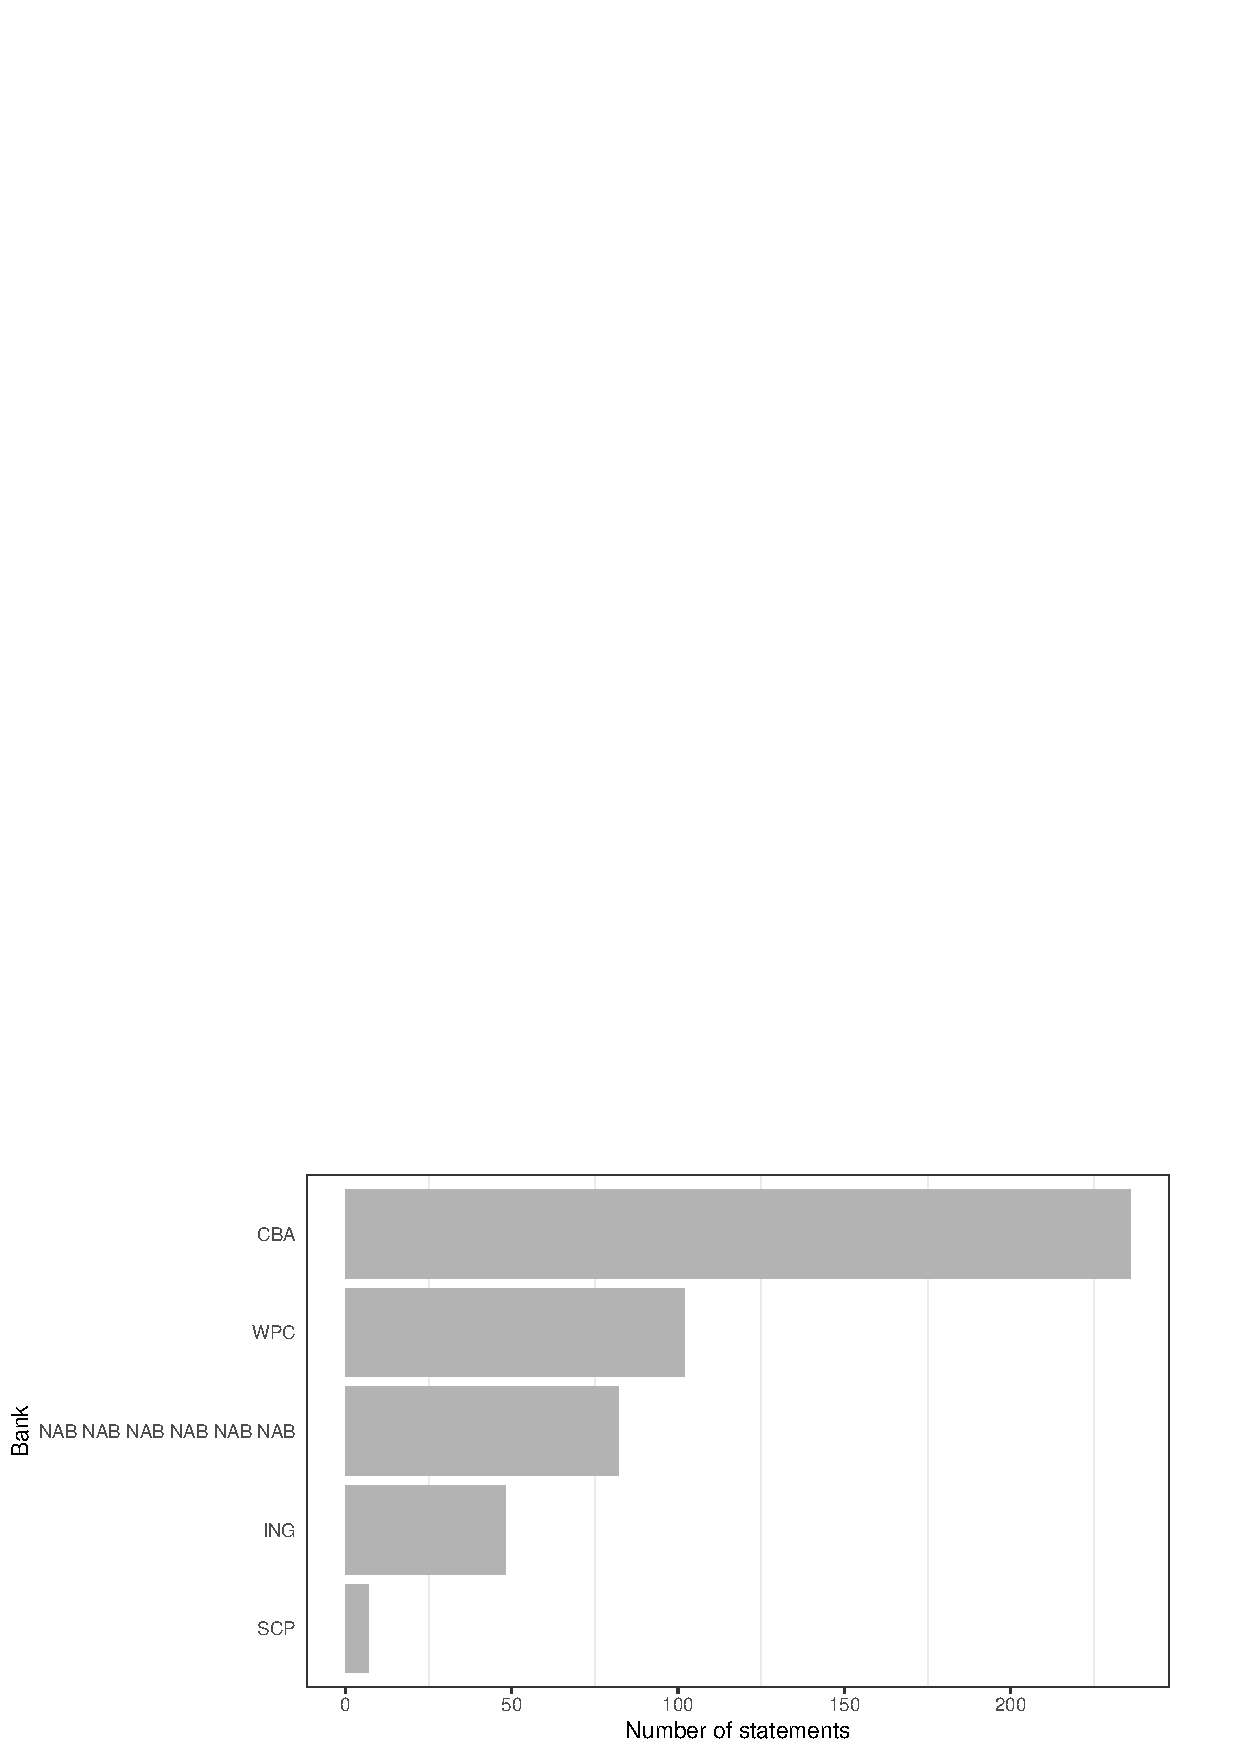
\includegraphics[width=\textwidth]{banks.pdf}
\caption{The distribution of statements for each bank.} \label{banks}
\end{figure}

These statements falls under 53 templates. 16 of which has only 1-2 samples.%, as shown in Fig.~\ref{templates}.
%\begin{figure}
%\includegraphics[width=\textwidth]{templates.pdf}
%\caption{The distribution of statements for each template.} \label{templates}
%\end{figure}

\subsection{Experiment Design}
Each of the vectoriser is applied with each classifier, making it 54 combinations to compare against our approach.

We have set aside 127 samples for test purposes. And used the remaining 348 to train model. We have ensured that for the minority classes, at least one sample remains in the training set.

We have employed a grid search technique on a diverse set of parameters and hyper-parameters of the algorithms employed 10-fold cross validation (CV) techniques for the machine learning models and 3-fold CV for the deep learning models to select the best parameters using the training set.

Once the best parameters are identified, we have induced a final model with the entire training set and evaluate the model on 127 test data.

To test the effect of the size of the training set, we have also used 53 samples to train each model and used the remaining data to test the model performance. We then continue to add 59 samples to the training data and check the model performance on the remaining data. Eventually, we have trained each model with 53, 112, 171, 230, 289 and 348 training data and test the model performance on the remaining. 

\section{Results}\label{result}
Add

\section{Discussion}\label{discuss}
Amin/Maruf to add

\section{Conclusion}\label{conc}
Maruf/Amin to add

%
% ---- Bibliography ----
%
% BibTeX users should specify bibliography style 'splncs04'.
% References will then be sorted and formatted in the correct style.
%
% \bibliographystyle{splncs04}
% \bibliography{mybibliography}
%
\bibliography{cm2.bib}{}
\bibliographystyle{splncs04}
\end{document}
